\documentclass[t, screen, aspectratio=43]{beamer}
\usepackage[T1]{fontenc}
\usepackage[utf8]{inputenc}
\usepackage{epsf}
\usepackage{graphicx}
\usepackage{geometry}
\usepackage{tabularx}
\usepackage[table]{colortbl}
\usepackage{xcolor}
\usepackage{soul}
\usepackage[normalem]{ulem}
\usepackage{tikz}
\usepackage{subcaption}
% Use the NTNU-temaet for beamer 
% \usetheme[style=ntnu|simple|vertical|horizontal, 
%     language=bm|nn|en, 
%     smalltitle, 
%     city=all|trondheim|alesund|gjovik]{ntnu2017}
\usetheme[style=helvet,language=en]{ntnu2017}

\usepackage[english]{babel}
\usepackage[style=numeric,backend=biber,natbib=false,sorting=none]{biblatex}

\title[Short title]{Ultra-Low Power PLL for Wake-up Receiver Applications}
\subtitle{Specialization Project Progress - 10th Week}
\author[C Nielsen]{Cole Nielsen}
\institute[NTNU]{Department of Electronic Systems, NTNU}
\date{1 November 2019 (Calendar week 44)}
%\date{} % To have an empty date

\addbibresource{example.bib} % Add bibliography database

% Set the reference style to numeric.
% See here: http://tex.stackexchange.com/questions/68080/beamer-bibliography-icon
\setbeamertemplate{bibliography item}[text] 

% Set bibliography fonts to a small size.
\renewcommand*{\bibfont}{\footnotesize}




\begin{document}

\begin{frame}
	\titlepage%
\end{frame}

% Alternatively, special title page command to get a different background
% \ntnutitlepage

% #############################################################################
% Timeline
% #############################################################################

\begin{frame}
	\frametitle{Timeline}
	\begin{table}[htb!]
		\tiny
		\centering
		\vspace{-1em}
		\def\arraystretch{1.5}		
		\setlength\arrayrulewidth{0.75pt}
		\setlength{\tabcolsep}{1em} % for the horizontal padding
		\begin{tabular}{|l|l|l|l|}
			\hline 
			\rule[-1ex]{0pt}{2.5ex} \cellcolor{gray!40}\textbf{Week} & \cellcolor{gray!40}\textbf{Dates} &\cellcolor{gray!40}\textbf{Tasks} & \cellcolor{gray!40}\textbf{Outcomes}\\ 
			\hline 
			\rule[-1ex]{0pt}{2.5ex} \cellcolor{red!20}\textbf{36}& \cellcolor{red!20}2.9 - 8.9 & \cellcolor{red!20}Review PLL Design & \cellcolor{red!20}Refreshed Knowledge\\ 
			\hline 
			\rule[-1ex]{0pt}{2.5ex} \cellcolor{red!20}\textbf{37}& \cellcolor{red!20}9.9 - 15.9 & \cellcolor{red!20}Modeling/simulation (set up) & \cellcolor{red!20}--\\ 
			\hline 
			\rule[-1ex]{0pt}{2.5ex} \cellcolor{red!20}\textbf{38}& \cellcolor{red!20}16.9 - 22.9 & \cellcolor{red!20}Modeling/simulation &\cellcolor{red!20}TDC/DCO Requirements\\ 
			\hline 
			\rule[-1ex]{0pt}{2.5ex} \cellcolor{red!20}\textbf{39}& \cellcolor{red!20}23.9 - 29.9& \cellcolor{red!20}Modeling/simulation& \cellcolor{red!20}Loop Filter/Digital Algorithms\\ 
			\hline 
			\rule[-1ex]{0pt}{2.5ex} \cellcolor{red!20}\textbf{40}& \cellcolor{red!20}30.9 - 6.10& \cellcolor{red!20}Modeling/simulation& \cellcolor{red!20}{Loop filter, DCO, TDC, calibration}\color{black}\\ 
			\hline 
			\rule[-1ex]{0pt}{2.5ex} \cellcolor{red!20}\textbf{41}&\cellcolor{red!20}7.10 - 13.10&\cellcolor{red!20}Circuit Research &\cellcolor{red!20}DCO/Divider topologies\\ 
			\hline 
			\rule[-1ex]{0pt}{2.5ex} \cellcolor{red!20}\textbf{42}&\cellcolor{red!20}14.10 - 20.10&\cellcolor{red!20}Circuit Research &\cellcolor{red!20}TDC/other topologies\\ 
			\hline 
			\rule[-1ex]{0pt}{2.5ex} \cellcolor{red!20}\textbf{43}&\cellcolor{red!20}21.10 - 27.10&\cellcolor{red!20}Spur analysis, filter automation &\cellcolor{red!20} \\ 
			\hline 
			\rule[-1ex]{0pt}{2.5ex}\cellcolor{green!20}\textbf{44}&\cellcolor{green!20}28.10 - 3.11&\cellcolor{green!20}Filter automation, SNR estimation&\cellcolor{green!20}\\ 
			\hline 
			\rule[-1ex]{0pt}{2.5ex} \textbf{45}& 4.11 - 10.11& Variation analysis, flicker noise & Histograms/yield estimates\\ 
			\hline 
			\rule[-1ex]{0pt}{2.5ex} \textbf{46}& 11.11 - 17.11& Real DCO sensitivity, TDC/divider jitter& Simlate ring-DCO in Virtuoso\\ 
			\hline 
			\rule[-1ex]{0pt}{2.5ex} \textbf{47}& 18.11 - 24.11& PLL + Radio simulation& BER estimate\\ 
			\hline 
			\rule[-1ex]{0pt}{2.5ex} \textbf{48}& 25.11 - 1.12& Agglomerate into cohesive framework & (I have an Exam on 30.11)\\ 
			\hline 
			\rule[-1ex]{0pt}{2.5ex} \textbf{49}& 2.12 - 8.12& Finish framework, report writing& \\ 
			\hline 
			\rule[-1ex]{0pt}{2.5ex} \textbf{50}& 9.12 - 15.12& Report writing& Complete before 15.12\\ 
			\hline 
		\end{tabular}
		\begin{flushleft}\textbf{Legend:} \colorbox{red!20}{\textbf{Done}} \colorbox{green!20}{\textbf{Current}}  \colorbox{blue!20}{\textbf{Revised}}
		% *I will write the report simultaneously with the work.
		\end{flushleft}
		% \caption{Assigned specifications for branch line hybrid design.}
		% \label{asgn_specs}
	\end{table}   
\end{frame}


% #############################################################################
% This week
% #############################################################################

\begin{frame}
	\frametitle{Timeline Tasks}
	\begin{block}{This week}
		\begin{itemize}
			\footnotesize
			\item \textbf{Filter design automation:}
			\begin{itemize}
				\footnotesize
				\item Was very slow, changed gradient-descent optimization approach.
			\end{itemize} 
			\item \textbf{Baseband SNR estimation}:
			\begin{itemize}
				\footnotesize
				\item Thought of way to estimate SNR of radio based on PLL phase noise and modulation PSD.
				\begin{itemize}
					\scriptsize
					\item Can determine BER based on radio system (modulation, bitrate and thus Eb/No)
				\end{itemize}			
				\item Utilize SNR estimate in optimization of PLL loop filter.
				\begin{itemize}
					\scriptsize
					\item Design to maximize received SNR.
				\end{itemize}	
			\end{itemize} 
		\item \textbf{Variation analysis:}
		\begin{itemize}
			\footnotesize
			\item Moved to next week due to SNR work.
		\end{itemize} 
		\end{itemize}    
	\end{block}
\end{frame}

% #############################################################################
% sim/modeling approach
% #############################################################################

\begin{frame}
	\frametitle{Filter automation}
	\begin{block}{Gradient descent optimization}
		\begin{itemize}
			\footnotesize
			\item Old approach used stepping method which tried to select optimal step size.
			\begin{itemize}
				\footnotesize
				\item Computing optimal step size is computationally expensive
				\item This method is actually slow than methods that use sub-optimal step size
			\end{itemize}
			\item Came across different method for selecting step size based \textit{only} on the gradient and cost function independent variables for current and previous iterations. 			
			\center
			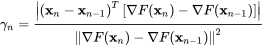
\includegraphics[width=0.4\linewidth]{gradstep.png}
			\begin{itemize}
				\footnotesize
				\item Very fast, despite using sub-optimal step size.
				\item Ca. 100x speed up in filter optimizer
			\end{itemize}

		\end{itemize}    
	\end{block}
\end{frame}

\begin{frame}
	\frametitle{Filter automation}
	\begin{block}{Gradient descent optimization}
		\begin{itemize}
		\footnotesize
		\item Now can optimize with many more iterations, matched closed loop response now is very close.
		\hspace{-20em}\begin{figure}[htb!]
	        \centering
	        \begin{subfigure}{0.4\textwidth}
	            \centering
	            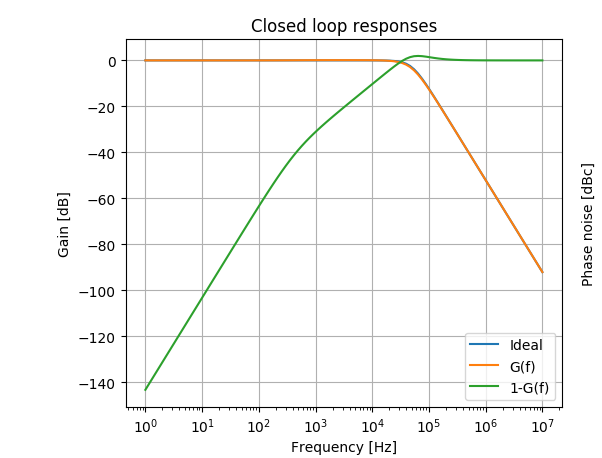
\includegraphics[width=0.9\linewidth]{tf_0707.png}
	            \caption{\scriptsize $\zeta$ = 0.707}
	            \label{fig:rosc_3stg_cir}
	        \end{subfigure}%
	        \begin{subfigure}{0.4\textwidth}
	            \centering
	            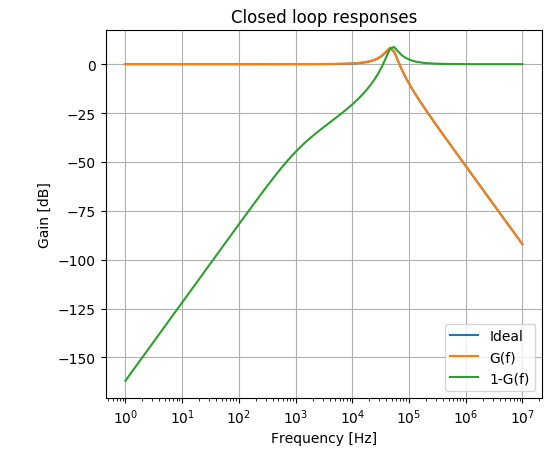
\includegraphics[width=0.9\linewidth]{tf_02.png}
	            \caption{\scriptsize $\zeta$ = 0.2}
	            \label{fig:rosc_3stg_wave}
	        \end{subfigure}
	        % \caption{Approximate model for ring oscillator inverter delay cell.}
	        \label{fig:rosc_3stg}
	    \end{figure}
		\end{itemize}    
	\end{block}
\end{frame}

\begin{frame}
	\frametitle{SNR estimation of radio with PLL}
	\begin{block}{Theory}
		\begin{itemize}
		\footnotesize
		\item Considering generalized PSK/FSK modulation in the phase domain, the phase of such a signal after direct-to-DC downconversion with local oscillator with phase noise $\phi_n(t)$ is:
		\begin{equation}
		\phi(t) = \phi_{mod}(t) + \phi_n(t)
		\end{equation}
		\item Given the mean of the phase noise $\langle\phi_n(t)\rangle$ = 0 and $|\phi_n(t)| <<$ 1, the amplitude of the signal can be approximated as:
		\begin{equation}
		\Re\{e^{\phi(t)}\} = \Re\{e^{\phi_{mod}(t)}e^{\phi_n(t)}\} \approx \Re\{e^{\phi_{mod}(t)}(1+j\phi_n(t))\}
		\end{equation}
		\begin{equation}
		= \cos(\phi_{mod}(t)) - \phi_n(t)\sin(\phi_{mod}(t))
		\end{equation}
		\item We can treat the downconverted signal in two parts, the main signal, $\cos(\phi_{mod}(t))$ (which is unchanged), and an orthogonal noise component that is the phase noise signal multiplied with a phase shifted version of the modulated signal ($\sin(\phi_{mod}(t))$). 
		\end{itemize}    
	\end{block}
\end{frame}


\begin{frame}
	\frametitle{SNR estimation of radio with PLL}
	\begin{block}{Application}
		\begin{itemize}
		\footnotesize
		\item In the frequency domain, the noise can be calculated as convolution of the modulated signal with the PLL phase noise
		\item The in band power then can be calculated for both the signal and noise to yield SNR:
		\center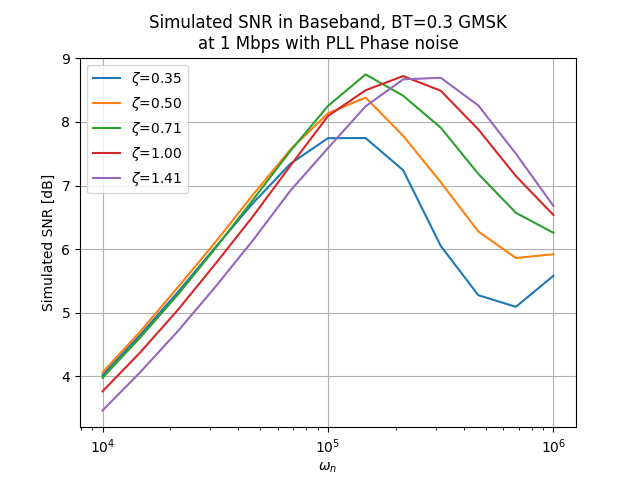
\includegraphics[width=0.6\linewidth]{snr.png}
		\end{itemize}    
	\end{block}
\end{frame}






% #############################################################################
% Loop Dynamics (continuous)
% #############################################################################

% \begin{frame}
% 	\frametitle{Loop Dynamics}
% 	\begin{block}{Still To Do}
% 		\vspace{-.2em}
% 		\begin{itemize}
% 			\footnotesize
% 			\item Standard approach to used mixed continuous/discrete time mathematical model for DPLL. 
% 			\item Plot of RO phase noise (typical)
% 			\item Automatic analysis of performance (lock detection, residual phase modulation, lock-in/pull-in range).
% 			\item Automatic optimization (using gradient descent) of PLL parameters?
% 			\item Z-domain modeling of loop? Develop (by hand) some ideal transfer funtions for loop.

% 		\end{itemize}    
% 	\end{block}
% \end{frame}

% #############################################################################
% Specification
% #############################################################################

\begin{frame}
	\frametitle{Specification (unchanged)\color{black}}
	\begin{block}{System Performance Targets}
		\scriptsize
		\begin{table}[h!]
			\centering
			\def\arraystretch{1.5}		
			\setlength\arrayrulewidth{0.75pt}
			\setlength{\tabcolsep}{1em} % for the horizontal padding
			\begin{tabular}{|l|r|l|l|}
				\hline 
				\rule[-1ex]{0pt}{2.5ex} \cellcolor{gray!40}\textbf{Parameter} & \cellcolor{gray!40}\textbf{Value} & \cellcolor{gray!40}\textbf{Unit }& \cellcolor{gray!40}\textbf{Notes}\\ 
				\hline 
				\rule[-1ex]{0pt}{2.5ex} \textbf{Frequency}  & 2.4-2.4835 & GHz & 2.4G ISM Band\\ 
				\hline 
				\rule[-1ex]{0pt}{2.5ex} \textbf{Ref. frequency} & 16 & MHz & Yields 6 channels \\ 
				\hline 
				\rule[-1ex]{0pt}{2.5ex} \textbf{Power} & $\leq$ 100  &$\mu$W & \\ 
				\hline 
				\rule[-1ex]{0pt}{2.5ex} \textbf{FSK BER} & $\leq$ 1e-2  & & 2FSK with $f_{dev}$=$\pm$250 KHz\\ 
				\hline 
				\rule[-1ex]{0pt}{2.5ex} \textbf{Initial Lock Time} & $\leq$ 50 & $\mu$s & Upon cold start \\ 
				\hline 
				\rule[-1ex]{0pt}{2.5ex} \textbf{Re-lock Time} & $\leq$ 5 & $\mu$s & Coming out of standby \\ 
				\hline 
				\rule[-1ex]{0pt}{2.5ex} \textbf{Bandwidth} & 50 & kHz & (nominally), tunable \\ 
				\hline 
			\end{tabular} 
			% \caption{Assigned specifications for branch line hybrid design.}
			% \label{asgn_specs}
		\end{table}   
		Additionally: PLL output should support IQ sampling at LO frequency.
	\end{block}    
\end{frame}

\begin{frame}
	\frametitle{Specification (unchanged)}
	\begin{block}{PLL Component Performance Targets}
		\scriptsize
		\begin{table}[h!]
			\centering
			\def\arraystretch{1.5}		
			\setlength\arrayrulewidth{0.75pt}
			\setlength{\tabcolsep}{1em} % for the horizontal padding
			\begin{tabular}{|l|r|l|l|}
				\hline 
				\rule[-1ex]{0pt}{2.5ex} \cellcolor{gray!40}\textbf{Parameter} & \cellcolor{gray!40}\textbf{Value} & \cellcolor{gray!40}\textbf{Unit }& \cellcolor{gray!40}\textbf{Notes}\\ 
				\hline 
				\rule[-1ex]{0pt}{2.5ex} \textbf{DCO LSB Resolution}  & $\leq$ 50  & kHz & Determined from quantization noise.\\ 
				\hline 
				\rule[-1ex]{0pt}{2.5ex} \textbf{DCO DNL} & < 1 & LSB & Ensures monotonicity \\ 
				\hline 
				\rule[-1ex]{0pt}{2.5ex} \textbf{TDC Resolution} & 0.95  & ns & \\ 
				\hline 
				\rule[-1ex]{0pt}{2.5ex} \textbf{TDC Resolution (bits)} &  6 &bits & \\ 
				\hline 
			\end{tabular} 
			% \caption{Assigned specifications for branch line hybrid design.}
			% \label{asgn_specs}
		\end{table}   
	\end{block}    
\end{frame}

% #############################################################################
% Architecture - block diagram
% #############################################################################

\begin{frame}
	\frametitle{Architecture (updated)}
	\begin{block}{Block Diagram}
	\center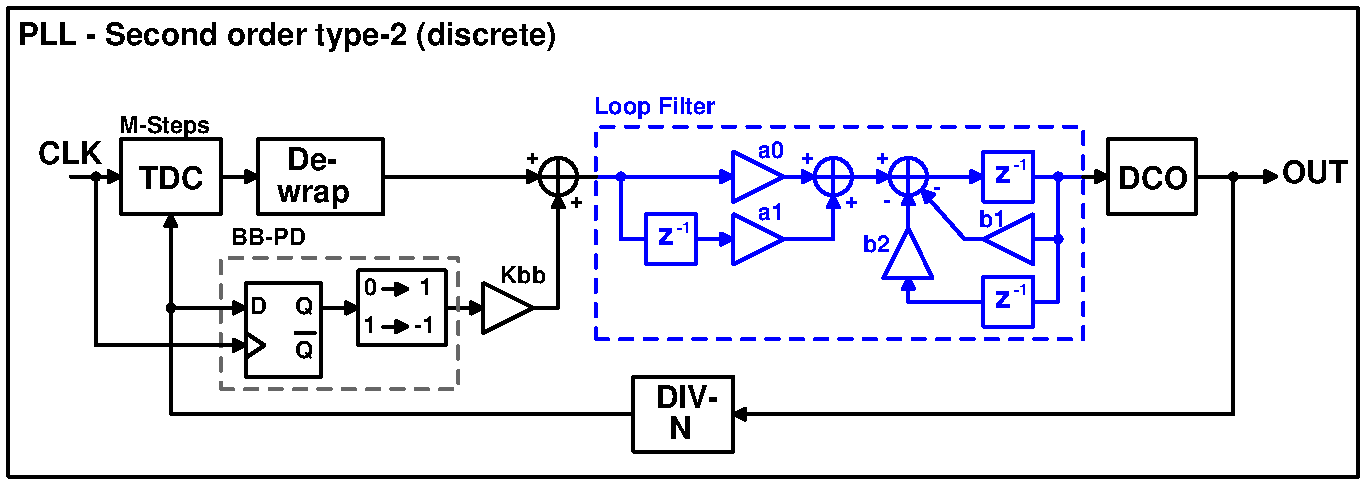
\includegraphics[width=0.8\textwidth, angle=0]{pll_sec_order_bb.pdf}

	\end{block}
		\begin{block}{Power Targets}
		\vspace{-.1em}
		\begin{table}[htb!]
			\tiny
			\centering
			\def\arraystretch{1.5}		
			\setlength\arrayrulewidth{0.75pt}
			\setlength{\tabcolsep}{1em} % for the horizontal padding
			\begin{tabular}{|l|l|l|l|l|}
				\hline 
				\rule[-1ex]{0pt}{2.5ex} \cellcolor{gray!40}\textbf{DCO} & \cellcolor{gray!40}\textbf{TDC} & \cellcolor{gray!40}\textbf{Divider }& \cellcolor{gray!40}\textbf{Other} & \cellcolor{gray!40}\textbf{SUM} \\ 
				\hline 
				\rule[-1ex]{0pt}{2.5ex} 70 $\mu$W& 20 $\mu$W & 10 $\mu$W & $<<$ 1 $\mu$W & 100 $\mu$W\\ 
				\hline 
			\end{tabular} 
			% \caption{Assigned specifications for branch line hybrid design.}
			% \label{asgn_specs}
		\end{table}   
	\end{block}

\end{frame}


% #############################################################################
% project phases
% #############################################################################


\begin{frame}
	\frametitle{Project Phases}
	\begin{block}{Autumn 2019}
		\footnotesize
		\begin{itemize}
			\item System modeling and simulation.
			\begin{itemize}
				\footnotesize
				\item Learn PLL theory in detail
				\item Evaluate feasability of PLL architectures (counter, TDC-based)
				\item Determine requirements for TDC/DCO/Divider/logic (bits of resolution, accuracy etc) to meet PLL performance specifications.
				\item Determine digital logic for loop filter, validate stability and lock time performance.
			\end{itemize}
			\item Research ultra-low power circuit topologies to implement system components that will meet determined requirements.
			\item Translate component-level specifications into schematic-level circuit designs.
			\begin{itemize}
				\footnotesize
				\item Try, fail, try again until functional at schematic level.
				\begin{itemize}
					\footnotesize
					\item I expect the TDC to be difficult.
				\end{itemize}
			\end{itemize}      
		\end{itemize}
	\end{block}
\end{frame}

% #############################################################################
% Project phases slide 2
% #############################################################################


\begin{frame}
	\frametitle{Project Phases (continued)}
	\begin{block}{Spring 2020}
		\begin{itemize}
			\footnotesize
			\item Finalize schematic-level design.
			\item Estabilish thorough tests for PLL performance (automated?) to help in layout.
			\item Layout of PLL.
			\begin{itemize}
				\footnotesize
				\item Design iteration until design specs met.
				\item Probably very time consuming.
			\end{itemize}
			\item Full characterization/validation of design performance. 
			\begin{itemize}
				\footnotesize
				\item Comprehensive Corners/Monte-Carlo testing (time consuming??)
				\item More design iteration if new issues crop up...
			\end{itemize}
			\item Thesis paper writing.
		\end{itemize}
	\end{block}
\end{frame}

% #############################################################################
% References
% #############################################################################


\begin{frame}
	\frametitle{References}
		\scriptsize
		[1] "Ultra-Low Power Wake-Up Receivers for Wireless Sensor Networks", N. Pletcher, J.M Rabaey, 2008.\\
		\hspace{16pt}\url{http://www.eecs.berkeley.edu/Pubs/TechRpts/2008/EECS-2008-59.html}\\
		\vspace{1em}
		% [2] "Minimum Achievable Phase Noise of RC Oscillators",
	% Navid et al. 2005
\end{frame}


\end{document}
